\section{Введение}
\subsection{Актуальность и значимость}

В целом если рассматривать приложения, которые взаимодействуют с блокчейном, то в последние несколько лет они несомненно являются актуальными и значимыми\cite{DBLP:journals/corr/abs-1712-04649}. В такой сфере вопрос об актуальности и значимости лучше делегировать на выбор блокчейна.

\begin{definition}
    Блокчейн --- децентрализованная база данных, которая содержит информацию о всех операциях произведенных в ней.
    Информация об операциях хранится в виде цепочки блоков.  Удалить или изменить цепочку блоков невозможно, все это защищено криптографическими методами. Самым первым блокчейном является Bitcoin\cite{nakamoto2012bitcoin}.
\end{definition}

Почему же NEAR Protocol является актуальным в нынешнее время? NEAR сеть обработала более 150 миллионов транзакций на текущий момент (28.05.2022 год). Для сравнения во время начала 2022 года количество обработанных транзакций оценивалось числом в 60 миллионов.
Активных аккаунтов в NEAR насчитывается более 12 миллионов штук (28.05.2022). На момент начала курсовой работы их было всего лишь 3 миллиона штук.

Несомненно выбор NEAR Protocol в качестве блокчейна является актуальным, потому что за менее чем 2 года он достиг таких цифр \cite{nearstats}.

\begin{figure}[H]
	\centering
	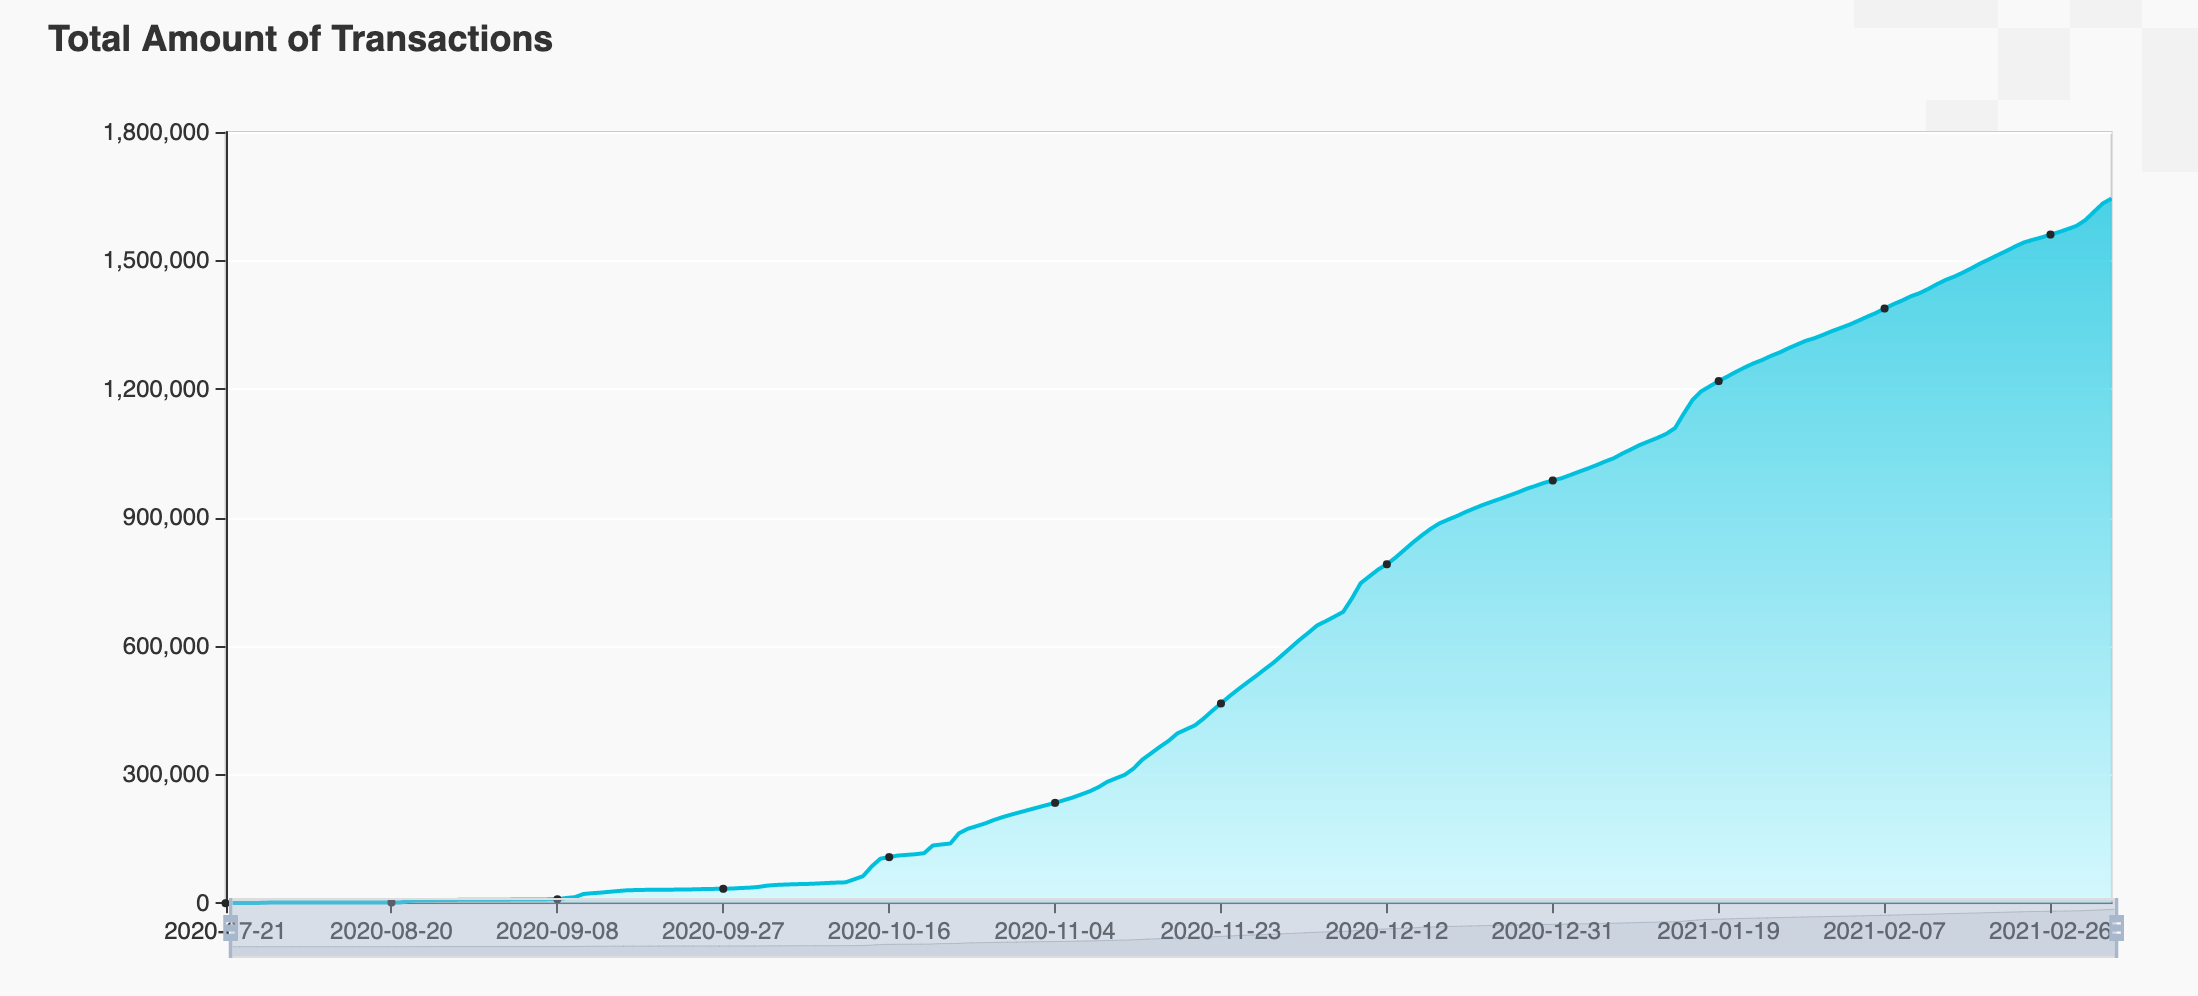
\includegraphics[height=60mm]{fig/near_1.png}
	\caption{Количество транзакций обработанных в NEAR Network}
\end{figure}


\begin{figure}[H]
	\centering
	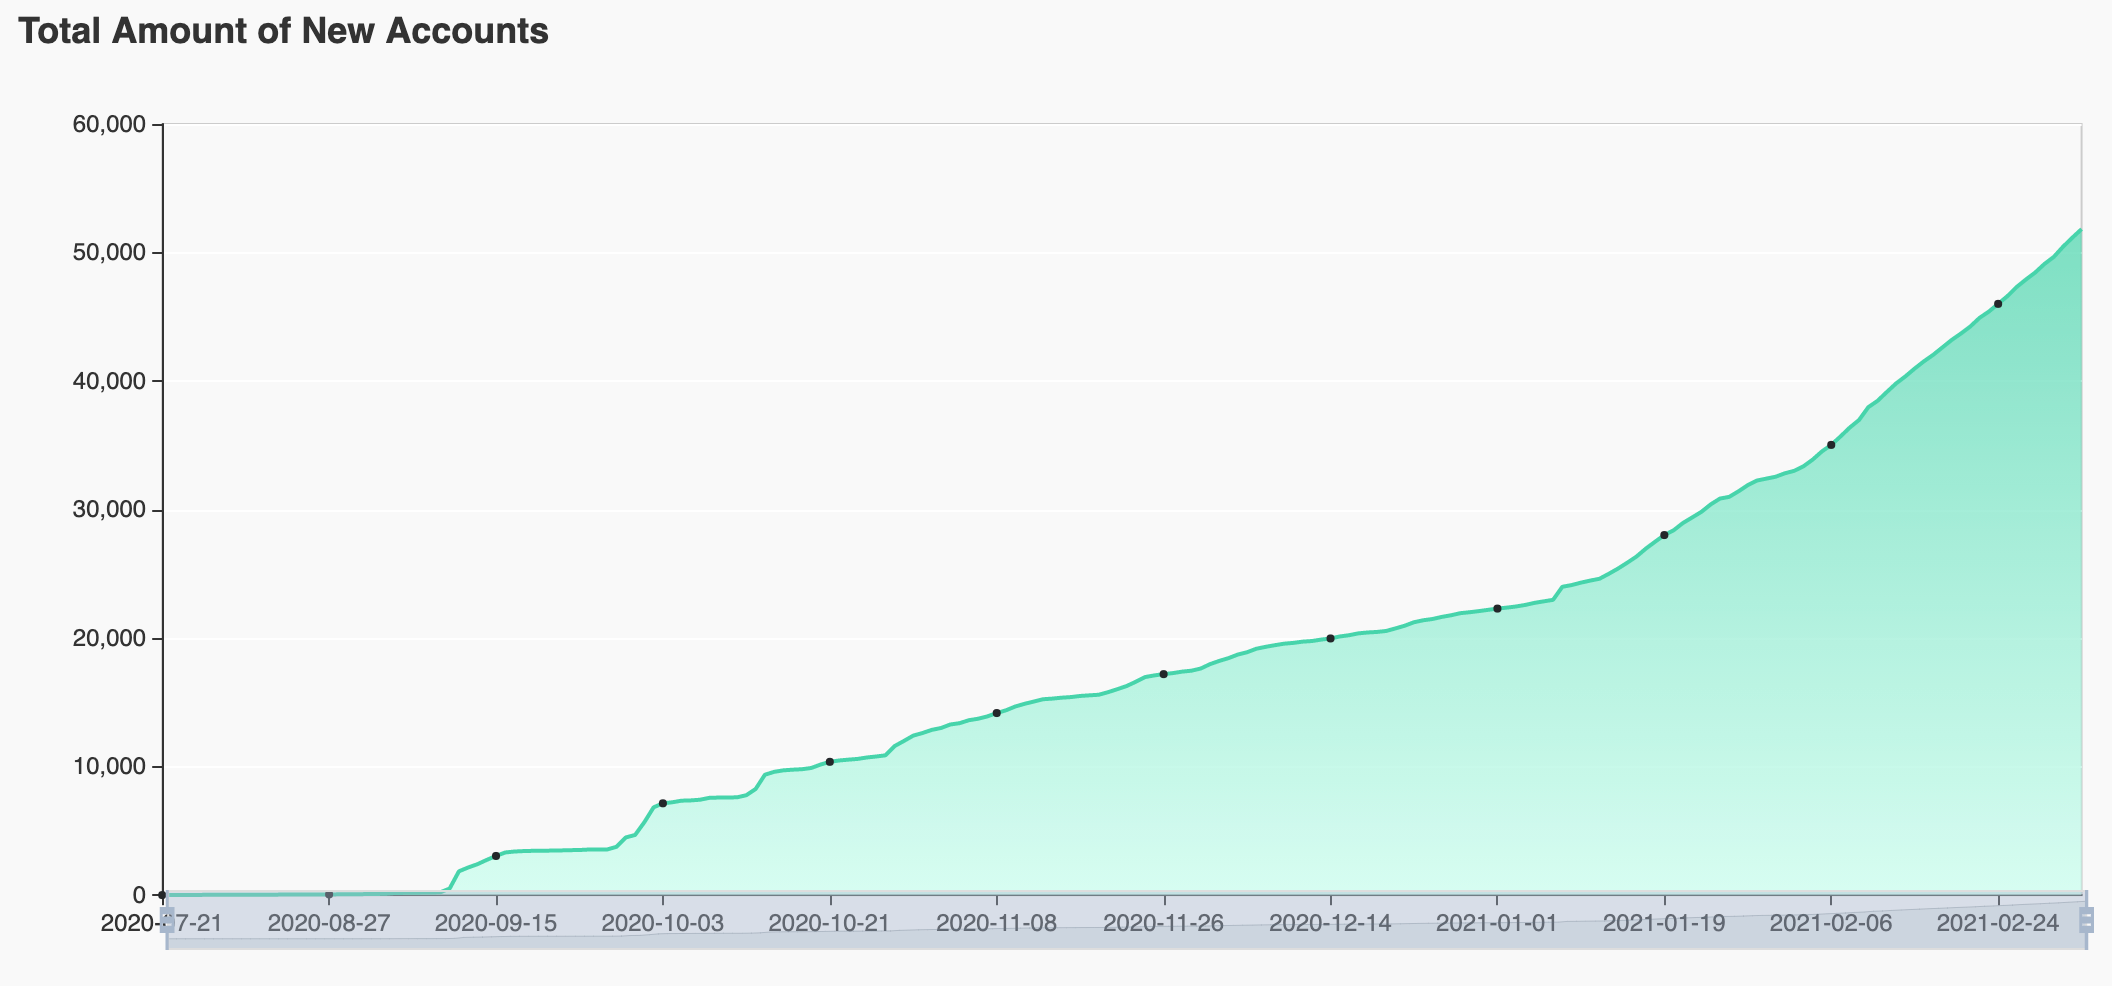
\includegraphics[height=60mm]{fig/near_2.png}
	\caption{Количество созданных кошельков в NEAR Network}
\end{figure}

Объяснение актуальности выбора самого приложения на базе блокчейна опирается на исследование Mapping the NFT revolution\cite{nftrevolution}. Авторы исследовали тренды 6.1 миллиона обменов в котором участвовало 4.7 миллиона NFT между 23 июнем 2017 и 27 апреля 2021. В заключении они утверждают, что: <<В целом, NFT новый инструмент, который удовлетворяет некоторые потребности создателей, пользователей и коллекционеров большого класса цифровых моделей. Как таковые, они, по крайней мере, и останутся или представляют собой начальный шаг к новым инструментам для работы с цифровой собственностью>>.

Почему именно наша реализация будет актуальной в сравнении с уже существующими решениями:


\begin{enumerate}
	\item Не существует еще ни одного полноценного NFT маркетплейса в Discord. Все существующие прототипы - это взаимодействие с API браузерных NFT маркетплейсов, который позволяют просто просматривать NFT токены, но не позволяют их создавать или обменивать, или продавать и так далее.
    Так как Discord - очень популярное приложение, API для построения бота, которого предоставляет очень широкий функционал, то выбор именно Discord по сравнению с аналогами Telegram или Slack.
	\item На данный момент не существует ни единого NFT маркетплейса, который встроил бы в себя функцию генерации NFT токена, используя генеративно-состязательную сеть. Мы хотим предоставить пользователю такую возможность, чтобы сэкономить время на придумывание NFT.
\end{enumerate}

\begin{definition}
    Discord - популярное приложение для группового чата, изначально было создано для того, чтобы дать геймерам место для создания сообществ и общения.
\end{definition}

\begin{definition}
    Генеративно-состязательная сеть (GAN) - это алгоритм машинного обучения, чьим основным элементом является состязательный процесс, в котором одновременно обучается две модели: генеративная модель G, которая пытается создать примеры имеющие схожее распределение с входными данными, и дискриминационная модель D, которая оценивает вероятность того, что выборка была получена из обучающих данных, а не сгенерирована генератором G\cite{generative_adversial_network}.
\end{definition}

Из вышеперечисленного утверждается, что NFT маркетплейс в блокчейне NEAR, предоставляющий интерфейс взаимодействия через Discord бота - соответствует нынешним трендам.


\subsection{Постановка задачи}
В качестве блокчейна используется NEAR protocol\cite{nearprotocol_2022}. NEAR Protocol работает по схеме Proof-of-Stake (Pos) \cite{nearprotocolpos}. Отличительные черты относительно других блокчейнов - улучшенная масштабируемость, производительность, а также простота реализации приложений.

\begin{definition}
    DApps --- это приложения, которые включают логику работы с функциями блокчейна\cite{ramamurthy2020blockchain}.
\end{definition}

Самой значимой частью реализации DApp являются Smart-контракты. Копии Smart-контрактов разворачивается с помощью специальной транзакции на всех узлах-участниках и исполняются в сети блокчейна.

\begin{definition}
    Smart-контракт --- это неизменяемый исполняемый код, представляющий логику DApp, работающий в блокчейне\cite{ramamurthy2020blockchain}. Часто сокращают до слова контракт. В некоторых протоколах называют по-другому, например в Solana - это программы\cite{solanaprogramlibrarydocs}.
\end{definition}

\begin{definition}
    Транзакция —-- это наименьшая единица работы, которая может быть назначена сети блокчейна. Работа в данном случае означает вычисление (выполнение функции) или хранение (чтение/запись данных)\cite{neardocumentationtransaction}.
\end{definition}

\begin{definition}
    Узлы-участники/валидаторы --- множество машин, которое обрабатывает транзакции в блокчейне.
\end{definition}

Для написания smart-контрактов NEAR protocol предоставляет sdk на языках Rust и AssemblyScript (near-sdk-rs\cite{nearsdkrs} и near-sdk-as\cite{nearsdkas} соответственно). В данном проекте smart-контракты NFT и маркетплейса реализовываются на языке Rust.

Discord-бот реализуется на языке программирования TypeScript, используя near-api-js\cite{nearapijs}. Discord-бот либо запускает <<view operations>> smart-контрактов, для получения метаданных привязанных к аккаунту; либо, при <<change operations>> создает транзакции с переданными аргументами пользователя и предоставляет URL для подписания транзакции пользователю. Discord API представляет множественный функционал для общения пользователя с ботом: slash-команды\cite{discordjsbuttons}, контекстные меню\cite{discordtscontextmenu}, меню выбора\cite{discordjsselectmenus}, кнопки\cite{discordjsbuttons}, модалы\cite{discordjsmodals}.


\begin{remark}
    Каждый smart-контракт в NEAR (написанный на Rust/Assembly Script) переводится в WebAssembly (Wasm), который исполняет виртуальная машина на участвующем узле (валидаторе) блокчейна. У smart-контракта, есть два вида функций: которые меняют состояние блокчейна - <<change operations>> и <<view operations>> - не меняют состояние блокчейна. Каждая транзакция имеет некоторое денежное обложение, которое измеряется в <<GAS>>. GAS - это сборы на исполнение транзакции, данные единицы - детерминированы, то есть одна и та же транзакция всегда имеет одинаковое обложение в GAS. Стоимость GAS пересчитывается в зависимости от загруженности сети в блокчейне \cite{neargas}.
\end{remark}

Для создания сервиса генерации NFT, необходимо обучить генеративную модель. Ее основной задачей будет являться генерация новых изображений, подобных тем, что имеются в тренировочном наборе данных. Данную модель можно получить используя генеративно-состязательную сеть.

Для связи дискорд бота с сервисом генерации NFT  с Discord-ботом необходимо разработать сервис, который будет возвращать URL для подписания транзакции на получение NFT. Нужно реализовать функционал, который позволяет получить случайный NFT, который не будет просматриваться в smart-контракте, чтобы пользователь не знал, какое NFT досталось ему до подписания транзакции. Сервис реализуется на языке Python с использованием фреймворка fast-api. Обращение к сервису реализуется с помощью http-запросов.

\subsection{Этапы проекта}
В рамках групповой курсовой работы была поставлена цель реализации discord-бота с функционалом NFT маркетплейса в NEAR protocol и сервисом генерации NFT, используя генеративно-состязательную сеть. Для реализации данной цели были выделены следующие этапы:
\begin{itemize}
    \item Изучить теоретический базис связанный с NEAR Protocol (Лущ, Басалаев, Токкожин, Кусиденов)
    \item Реализовать smart-контракты (Басалаев):
    \begin{itemize}
        \item Изучить язык Rust для написания smart-контрактов;
        \item Изучить стандарт NFT токенов;
        \item Реализовать core функционал NFT токенов - mint (создание) NFT и отправка между пользователями;
        \item Реализовать enumeration функции - получение списка токенов, используя pagination;
        \item Реализовать Approval Management внутри структуры NFT;
        \item Поддержать Royalties - распределение доходов от продажи NFT среди нескольких аккаунтов в соотношение с долями;
        \item Покрыть основную часть функционала NFT smart-контракта тестами;
        \item Изучить существующие решения маркетплейс контрактов, подчеркнуть из них самое полезное;
        \item Организовать функции покупки хранилища под продажу NFT токенов;
        \item Написать функцию возвращения NEAR за неиспользуемое хранилище для продажи NFT токенов;
        \item Реализовать функцию выставления на продажу в маркетплейс smart-контракте;
        \item Добавить enumeration функции - получение списка продаваемых токенов, используя pagination;
        \item Реализовать изменение цены/отмену продажи для выставленного на маркетплейс NFT токена;
        \item Добавить возможность покупку продаваемых на маркетплейсе NFT токенов;
        \item Покрыть основную часть функционала маркетплейс smart-контракта тестами;
    \end{itemize}
    \item Разработать discord-бота (Лущ):
    \begin{itemize}
        \item Изучить Javascript/Typescript;
        \item Изучить основы работы с браузером через Javascript (сессионное/локальное хранилище браузера, класс window);
        \item Изучить near-api-js и его кода для дальнейшего его переписывания под функциональность discord;
        \item Реализовать KeyStore\cite{nearclasskeystore} работающий через Redis\cite{redis};
        \item Написать реализацию авторизации в NEAR Wallet\cite{nearwallet} через discord-бота, который использует вышеописанный KeyStore;
        \item Написать реализацию создания URL на подпись транзакции/транзакций (одна транзакция\footnote{В данном контексте класс Transaction\cite{nearclasstransaction}}, один Action\cite{nearclassaction}; одна транзакция, несколько Action; несколько транзакций, несколько Action);
        \item Создание <<Профиля пользователя>>. Вызов осуществляется через slash-команду\cite{discordjsslashcommands} или контекстное меню;
        \item Реализация просмотра списка NFT, которыми владеет пользователь, которые продает пользователь, которые продаются на всем маркетплейсе. Вызовы осуществляются через контекстные меню, slash-команды, кнопки в профиле пользователя;
        \item Поддержка покупки, продажи, отмены продажи NFT. Вызовы в виде кнопок при просмотре NFT списка;
        \item Изучение децентрализованных распределенных хранилищ;
        \item Реализация mint (создания) NFT с использованием децентрализованных распределенных хранилища;
        \item Поддержка изменения цены NFT;
        \item Поддержать сервис c генеративно-состязательной сетью в discord-боте;
        \item Сделать docker образ для удобного деплоя discord-бота;
        \item Деплой discord-бота на облачный сервис (Кусиденов);
    \end{itemize}
    \item Реализовать генеративно-состязательную сеть (Токкожин):
    \begin{itemize}
        \item Обработка тренировочного набора данных;
        \item Написать архитектуру модели генератора;
        \item Написать архитектуру модели дискриминатора;
        \item Обучение моделей;
        \item Улучшение качества изображений генерируемых моделью путем изменения гиперпараметров нейронных сетей;
        \item Написание скрипта для простой генерации картинки, способствующей созданию сервиса;
        \item Добавить теги к генерируемому изображению, для их дальнейшей передачи в качестве атрибутов;
    \end{itemize}
        \item Реализовать сервис с генеративно-состязательной сетью (Кусиденов):
    \begin{itemize}
    	\item Изучить как связать бота с сервисом и обсудить требования;
    	\item Продумать как скрыть сгенерированное NFT для пользователя маркетплейса;
    	\item Реализовать сервис, который по запросу бота будет отдавать NFT с его характеристиками;
    	\item Реализовать контракт, который скрывает какое NFT достанется пользователю.
    \end{itemize}
\end{itemize}

\subsection{Структура работы}

Работа организована следующим образом. В разделе {\color{blue} \ref{section.theory}} дается обзор существующих на сегодняшний день маркетплейсов на NEAR Protocol. Раздел {\color{blue} \ref{section.main.smart}} описывает устройство и реализацию smart-контрактов NFT и маркетплейса. В {\color{blue} \ref{section.main.bot}} разделе идет описание трудностей и их решения в разработке discord-бота. В {\color{blue} \ref{section.generative_adversial_network}} разделе описывается ход работы над генеративно-состязательною сетью. В {\color{blue} \ref{section.ganservice}} разделе описывается сервис генерации NFT и его взаимодействие с discord-ботом.
Конечные результаты и планы на дальнейшую работу можно найти в разделе {\color{blue} \ref{section.output}}.
